\title{Solid State Physics: Midterm 2 Review}

\documentclass[10pt]{article}
\usepackage{amsthm}
\usepackage{graphicx}
\usepackage{subfig}
\usepackage{physics}
\graphicspath{ {figures/} }
\begin{document}
\maketitle


\section{One-dimensional Monatomic Chain}
Consider a chain of identical atoms of mass $m$ and lattice spacing $a$. The position of the $n$th atom is $x_{n}$
and the equilibrium position of the $n$th atom is $x_{n}^{eq} = na$. Deviations from the equilibrium position are
expressed as $\delta x_{n}$ where
$$\delta x_{n} = x_{n} - x_{n}^{eq} $$
The total potential energy of the chain is
$$V = \sum_{i} = \frac{1}{2}\kappa(x_{i+1}-x_{i}-a)^{2} = \sum_{i}\frac{1}{2}\kappa(\delta x_{i+1} - \delta x_{i})^{2}$$
The force on the $n$th mass of the chain is
$$F_{n} = -\frac{\partial V}{\partial x_{n}} = \kappa(\delta x_{n+1} - \delta x_{n}) + \kappa(\delta x_{n-1} - \delta x_{n})$$
From this we obtain Newton's equation of motion
$$m(\delta \ddot{x}_{n}) = F{n} =  \kappa(\delta x_{n+1}+ \delta x_{n-1} - 2\delta x_{n})$$

\begin{itemize}
  \item A \emph{normal mode} is defined to be a collective oscillation where all particles move at the same frequency.
  \item Ansatz solution to equation of motion:
  $$\delta x_{n} = Ae^{i\omega t - ikx_{n}^{eq}} = Ae^{i\omega t - ikna}$$
  where $A$ is the amplitude of oscillation, and $k$ and $\omega$ are the wavevector and frequency of the proposed wave.
  \item Even though the solution is complex, we are implicitly meant to take the real part. We only need to consider $\omega \geq 0$
  but $k$ can be positive or negative.
\end{itemize}

Plugging the ansatz into the equation of motion yields
$$m\omega^{2} = 2\kappa\left [ 1-\cos(ka)\right] = 4\kappa \sin^{2}(ka/2)$$
and therefore
$$\omega = 2\sqrt{\frac{\kappa}{m}} \left | \sin(\frac{ka}{2})\right |$$
which is the \emph{dispersion relation} - defined as the relationship between frequency (or energy) and a wavevector (or momentum).

\begin{figure}
  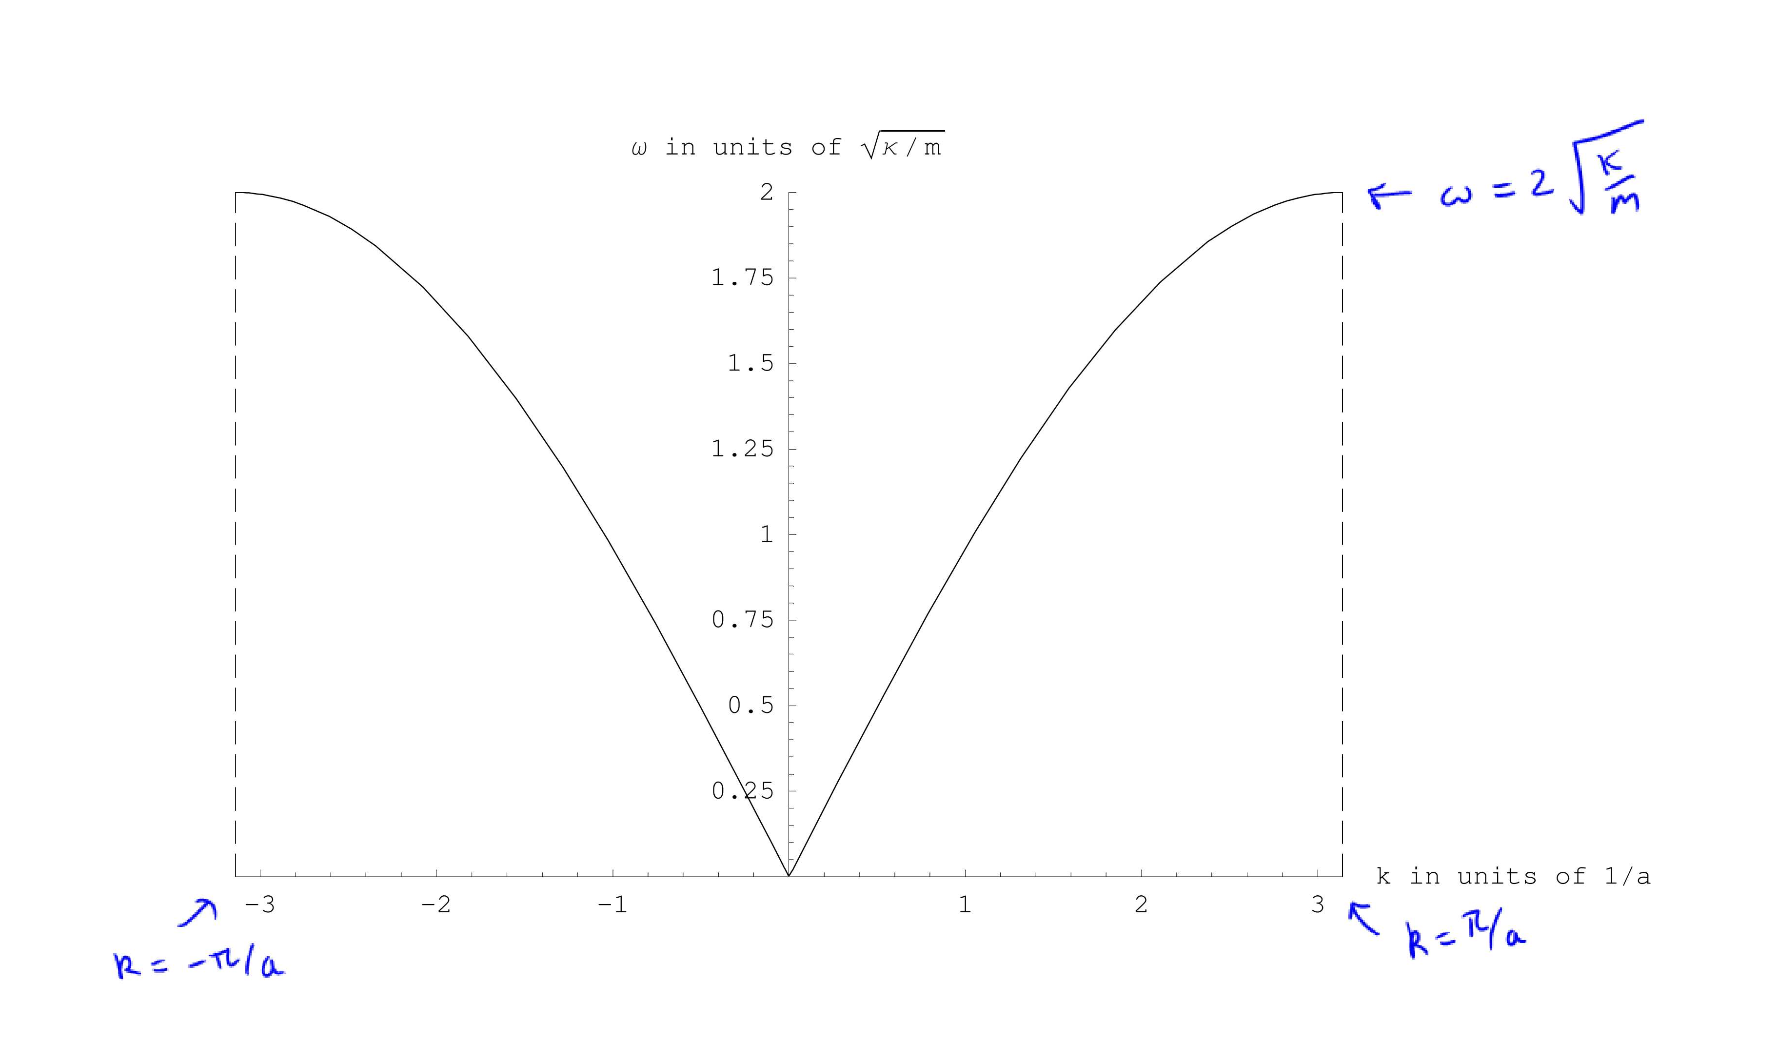
\includegraphics[width=\linewidth]{1d_disp.png}
  \caption{Dispersion relation for 1D monatomic chain.}
\end{figure}

\subsection{Reciprocal Lattice}
The dispersion relation in Fig. 1 is periodic in $k \rightarrow k + 2\pi/a$. An important
general principle is the following: \emph{A system which is periodic in real space with a periodicity
$a$ will be periodic in reciprocal space with periodicity $2\pi/a$}. In other words, if the system "looks
the same" when $x \rightarrow x + a$, then the dispersion will look the same when $k \rightarrow k + 2\pi/a$.


The periodic unit in $k$-space is known as the \emph{Brillouin zone}. The \emph{first Brillouin zone} is centered about $k = 0$.
The points $k = \pm \pi/a$  in Fig. 1 are known as the \emph{Brillouin zone boundary}.


If we take $k \rightarrow k + 2\pi p/a$, where $p$ is any integer, then our solution for $\delta x_{n}$ will not change since it is
a deep fact that
$$e^{i2\pi n p} = 1$$
The \emph{reciprocal lattice} is therefore defined as a set of point in $k$-space (\emph{reciprocal space}) which are physically
equivalent to the point $k = 0$. The set of points $x_{n}$ are known as the \emph{direct lattice} or \emph{real-space lattice}.

As an example, the points in the direct lattice of the one-dimensional monatomic chain with lattice spacing $a$ are
$$x_{n} = ..., -2a, -a, 0, a, 2a, ...$$
and the reciprocal lattice points are
$$G_{n} = ..., -2\left (\frac{2\pi}{a} \right), -\left (\frac{2\pi}{a} \right), 0, \left (\frac{2\pi}{a} \right), 2\left (\frac{2\pi}{a} \right),... $$
And the defining property of the reciprocal lattice points are:
\begin{equation}
  \boxed{e^{iG_{m}x_{n}} = 1}
\end{equation}
That is, a point $G_{m}$ is in the reciprocal lattice only if the above holds for all $x_{n}$ in the direct lattice.
An important note: $k$ and $k+G_{m}$ only describe the same wave when measured at direct lattice points $x_{n}$. If measured arbitrarily
along the x-axis, they may differ.

\subsection{Sound Waves}
Sound waves are vibrations with a long wavelength compared to the interatomic spacing. That is, $k = \frac{2\pi}{\lambda}$, where $\lambda >> a$.
Therefore, the dispersion becomes
$$\omega = v_{sound}k = \left ( a \sqrt{\frac{\kappa}{m}}\right)k$$
At larger $k$ (shorter $\lambda$), the dispersion is no longer linear and one typically defines two velocities.
\begin{itemize}
  \item The group velocity $v_{group} = d\omega /dk$. The speed at which the wavepacket moves. The group velocity becomes 0 at the Brillouin zone boundary.
  \item The phase velocity $v_{phase} = \omega / k$. The speed at which individual minima/maxima move.
\end{itemize}

\subsection{Counting Normal Modes}
At first glance, it would appear that any choice of $k$ in the first Brillouin zone yields a unique normal mode with frequency $\omega(k)$.
But periodic boundary conditions imply that $x_{n} = x_{n + N}$. This yields the requirement in our solution that
$$e^{ikNa} = 1$$
From which we obtain the restriction on possible values of $k$:
$$k = \frac{2\pi m}{Na}$$
where $m$ is some integer. So the full dispersion relation only contain several allowed $k$ values, the spacing between which is $2\pi/Na$.
The total number of normal modes is therefore given by the range of the Brillouin zone (e.g. $[-\pi/a,\pi/a]$), divided by the spacing between
allowed normal mode values of $k$. Be careful to only include one endpoint in the Brillouin zone.

\subsection{Quantum Phonons}
Quantum correspondance: If a classical harmonic system has a normal oscillation mode at frequency $\omega$ the corresponding
quantum system will have eigenstates with energy
$$E_{n} = \hbar \omega (n + \frac{1}{2})$$
\begin{itemize}
\item At a given wavevector $k$ there are many possible eigenstates.
\item The ground state is the $n = 0$ state with zero point energy $\hbar \omega(k)/2$.
\item All excitations occur in units of $\hbar \omega(k)$.
\end{itemize}
A \emph{phonon} is a discrete quantum of vibration, and corresponds to an excitation of the normal mode by increasing the
quantum number $n$.
\begin{itemize}
  \item Phonons are bosons. We may think of them as particles with energy $\hbar \omega$ and \emph{crystal} momentum $\hbar k$. We always describe
  momentum using $k$ within the first Brillouin zone. Even though $k$ is equivalent to $k + G_{m}$, they do not describe the same momentum.
  \item At finite temperature, there are non-zero number of phonons occupying a given mode, described by the Bose occupation factor:
  $$n_{B}(\beta \hbar \omega) = \frac{1}{e^{\beta \hbar \omega} - 1}$$
  \item The expectation value of energy of phonons at wavevector $k$ is given by
  $$E_{k} = \hbar \omega(k) \left (n_{B}(\beta \hbar \omega) + \frac{1}{2} \right )$$
  \item The total energy is given by
  $$U_{tot} = \sum_{k} E_{k}$$
  where the sum is over all possible normal modes (i.e. $\frac{-\pi}{a} < k \leq \frac{\pi}{a}$, such that $k = \frac{2\pi m}{Na}$).
  When the system is very large, the spacing between normal modes shrinks, and we may convert the sum into an integral.
  $$\sum_{k} \rightarrow \frac{Na}{2\pi}\int_{-\pi/a}^{\pi/a}dk$$.
  \item We also note that the total number of normal modes is given by
  $$\frac{Na}{2\pi}\int_{-\pi/a}^{\pi/a}dk$$
  \item From the integral form of $U_{tot}$, we could calculate the heat capacity
  $$C = \frac{dU}{dT}$$
  \item This approach is identical to the Debye model, except that Debye assumed $\omega = vk$, whereas our dispersion
  relation is much more complicated.
  \item We may also convert the integral over $k$ to an integral over $\omega$ by introducing a density of states $g(\omega)$.
  $$\frac{Na}{2\pi}\int_{-\pi/a}^{\pi/a}dk = \int d\omega g(\omega)$$
  $$g(\omega) = 2 \frac{Na}{2\pi}\left | \frac{dk}{d\omega}\right |$$
\end{itemize}

\section{Vibrations of the One-Dimensional Diatomic Chain}
Consider a one-dimensional chain of alternating masses $m_{1}$ and $m_{2}$ with alternating connecting spring constants $\kappa_{1}$ and $\kappa_{2}$.
The unit cell for the diatomic chain consists of both masses and is of length (lattice constant) $a$. It is useful to pick a reference point for each unit
cell, the set of these reference points forms a simple lattice. Within each unit cell, the individual atoms in the cell are described relative to the reference
point - this description forms the basis.

\subsection{Normal Modes}
Assume for now that $m_{1} = m_{2} = m$. The equations of motion follow from the monatomic case. But now, let $x_{n}$ be the position of the $n$th $m_{1}$
mass and $y_{n}$ be the position of the $n$th $m_{2}$ mass. Let $\kappa_{1}$ connect $y_{n}$ to $x_{n+1}$.
$$m\ddot{\delta x_{n}} = \kappa_{2}(\delta y_{n} - \delta x_{n}) + \kappa_{1}(\delta y_{n-1} - \delta x_{n})$$
$$m\ddot{\delta y_{n}} = \kappa_{1}(\delta x_{n+1} - \delta y_{n}) + \kappa_{2}(\delta x_{n} - \delta y_{n})$$
The ansatz solutions will be
$$\delta x_{n} = A_{x}e^{i \omega t - ikna}$$
$$\delta y_{n} = A_{y}e^{i \omega t - ikna}$$
\begin{itemize}
  \item Because the lattice spacing is $a$, $k$ is physically equivalent to $2\pi/a$, so the first Brillouin zone is defined by
  $$-\pi/a \geq k \leq \pi/a$$
  \item For $N$ unit cells, such that the system length is $L = Na$, the allowed values of $k$ are
  $$k = \frac{2\pi m}{Na} = \frac{2 \pi m}{L}$$
  \item The number of possible $k$ values is $N$ - one value of $k$ per unit cell.
  \item Debye's intuition: there should be one mode per degree of freedom. We have $2N$ degrees of freedom, but $N$ values of $k$. Resolution:
  there are two modes per $k$ value.
\end{itemize}

Plugging in the ansatz solutions to the equations of motion yields
$$-\omega^{2}mA_{x} = \kappa_{2}A_{y} + \kappa_{1}A_{y}e^{ika} - (\kappa_{1} + \kappa_{2})A_{x}$$
$$-\omega^{2}mA_{y} = \kappa_{1}A_{x}e^{-ika} + \kappa_{2}A_{x} - (\kappa_{1} + \kappa_{2})A_{y}$$

This can be written as
$$
m\omega^{2} \begin{bmatrix}
A_{x}\\ A_{y}
\end{bmatrix} =
\begin{bmatrix}
 (\kappa_{1} + \kappa_{2})& -\kappa_{2} - \kappa_{1}e^{ika}\\
-\kappa_{2}-\kappa_{1}e^{-ika} & (\kappa_{1} + \kappa_{2})
\end{bmatrix}
\begin{bmatrix}
A_{x}\\ A_{y}
\end{bmatrix}
$$

The solutions are obtained by finding the zeroes of the characteristic determinant.
$$
0 = \begin{vmatrix}
 (\kappa_{1} + \kappa_{2}) - m\omega^{2}& -\kappa_{2} - \kappa_{1}e^{ika}\\
-\kappa_{2}-\kappa_{1}e^{-ika} & (\kappa_{1} + \kappa_{2})-m\omega^{2}
\end{vmatrix}
$$

The roots are given by
$$
m\omega^{2} = (\kappa_{1} + \kappa_{2}) \pm \left | \kappa_{1} + \kappa_{2}e^{ika}\right |
$$
which can be written as
$$
\omega^{2} = \frac{(\kappa_{1} + \kappa_{2})}{m} \pm \frac{\sqrt{\kappa_{1}^{2} + \kappa_{2}^{2} + 2\kappa_{1}\kappa_{2}cos(ka)}}{m}
$$
The $\pm$ in the dispersion indicates that there are two branches of the dispersion for each $k$ value - and therefore $2N$ normal modes
in total. 

\section{Crystal Structure}
\subsection{Basics of Crystal Structure}
\begin{itemize}
\item A \emph{lattice} is an infinite set of points defined by integer sums of a set of linearly
independent \emph{primitive lattice vectors}.
\item Alternatively: A \emph{lattice} is an infintie discrete set of vectors where addition of
any two vectors in the set gives a third vector in the set, or a \emph{lattice} is an infinite
discrete set of points where the environment of any given point is equivalent to the environment
of any other point.
\item Lattice points may be described in three dimensions as
$$\textbf{R} = n_{1}\textbf{a}_{1} + n_{2}\textbf{a}_2 + n_{3}\textbf{a}_{3}$$
\item In 2+ dimensions, the choice of primitice lattice vectors is not unique.
\end{itemize}

\begin{itemize}
  \item A \emph{unit cell} is the repeated motif which is the elementary building block of
  any periodic structure. When many identical unit cells are tiled together, they
  completely fill all of space and reconstruct the full structure.
  \item A \emph{primitive unit cell} is a unit cell containing exactly one lattice point.
  \item A \emph{conventional unit cell} is a typically less-minimal unit cell, often
  with orthogonal axes, chosen due to ease of use.
  \item A \emph{Wigner-Seitz cell} is constructed by including all points in space that are
  closer to a given lattice point than any other lattice point. Approach: choose a lattice cell
  and draw lines to all possible neighbors. Perpendicular bisectors of these lines bound the
  Wigner-Seitz cell.
  \item The description of the unit cell with respect to the associated lattice point is
  known as the \emph{basis}.
  \item The positions of atoms can be described by
  $$ \textbf{R} = \textbf{R}_{lattice} + \textbf{R}_{basis} $$
  \item The \emph{coordination number} of a lattice is the number of nearest neighbors to any point of the lattice.
\end{itemize}

\subsection{Three-Dimensional Lattices}
The simplest example is the \emph{simple cubic} lattice.
\begin{itemize}
  \item The primitive unit cell is typically a cube, where each corner contributes $1/8$ lattice point.
  \item \emph{Tetragonal} and \emph{orthorhombic} lattices have two and three different primitive lattice
  vector lengths, respectively.
  \item A point in the lattice may be written as $[uvw]$ where
  $$[uvw] =  u\textbf{a}_{1} + v\textbf{a}_2 + w\textbf{a}_{3}$$
  \item In the case of orthogonal axes, $\textbf{a}_{1}$ is assumed to be in the $\hat{x}$ direction, etc.
\end{itemize}

The \emph{body-centered cubic} lattice is identical to the simple cubic lattice, but with an additional
lattice point in the center of the cube.
\begin{itemize}
  \item The conventional unit cell contains $8(1/8) + 1 = 2$ lattice points.
  \item The points of the BCC lattice can be written as
  $$\textbf{R}_{corner} = [n_{1}, n_{2}, n_{3}]$$
  $$\textbf{R}_{center} = [n_{1}, n_{2}, n_{3}] + [1/2, 1/2, 1/2]$$
  \item We can also think of the BCC as two interpenetrating SC lattices, displaced by $[1/2, 1/2, 1/2]$.
  \item The coordination number $Z = 8$.
  \item One choice of primitive lattice vectors:
  $$\textbf{a}_{1} = [1, 0, 0]$$
  $$\textbf{a}_{2} = [0, 1, 0]$$
  $$\textbf{a}_{3} = [1/2, 1/2, 1/2]$$

\end{itemize}

The \emph{face-centered cubic} lattice is similar to the simple cubic lattice, but with the addition of a
lattice point on every cube face.
\begin{itemize}
\item The conventional unit cell contains $8(1/8) + 6(1/2) = 4$ lattice points.
\item The points of the FCC lattice can be written as
$$\textbf{R}_{corner} = [n_{1}, n_{2}, n_{3}]$$
$$\textbf{R}_{xy} = [n_{1}, n_{2}, n_{3}] + [1/2, 1/2, 0]$$
$$\textbf{R}_{yz} = [n_{1}, n_{2}, n_{3}] + [0, 1/2, 1/2]$$
$$\textbf{R}_{zx} = [n_{1}, n_{2}, n_{3}] + [1/2, 0, 1/2]$$
\item We can also think of the FCC as four interpenetrating SC lattices, displaced as described above.
\item One choice of primitive lattice vectors:
$$\textbf{a}_{1} = [1/2, 1/2, 0]$$
$$\textbf{a}_{2} = [1/2, 0, 1/2]$$
$$\textbf{a}_{3} = [0, 1/2, 1/2]$$
\end{itemize}

\section{Reciprocal Lattice, Brillouin Zone, Waves in Crystals}


\section{Misc}
\begin{itemize}
  \item $$\sin(x) = \frac{e^{ix} - e^{-ix}}{2i}$$
  \item $$\cos(x) = \frac{e^{ix} + e^{-ix}}{2}$$
  \item $$\sin^{2}(x) = \frac{1 - \cos(2x)}{2}$$
  \item $$\cos^{2}(x) = \frac{1 + \cos(2x)}{2}$$
\end{itemize}
\end{document}
